
\usetikzlibrary{decorations.markings}

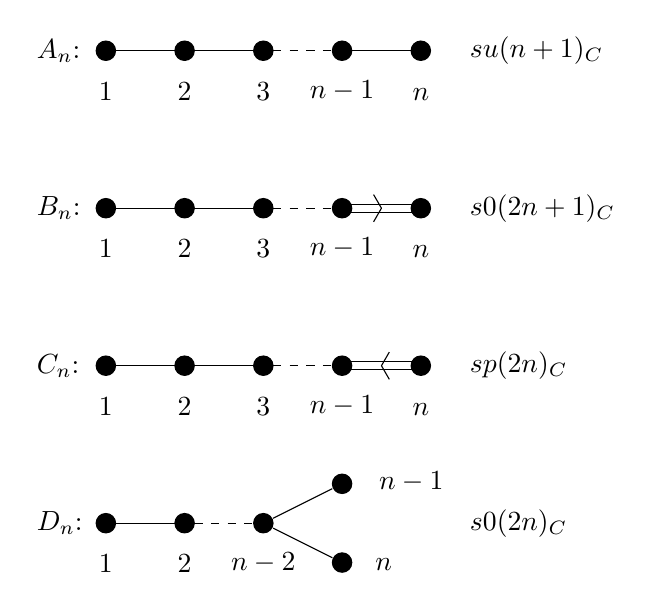
\begin{tikzpicture}

%-------------- An -------------------------------
  
\node [label={[yshift=-25pt]1}] (A1) at (-5,0) {};
\node [label={[yshift=-25pt]2}] (A2) at (-4,0) {};
\node [label={[yshift=-25pt]3}] (A3) at (-3,0) {};
\node [label={[yshift=-25pt]$n-1$}] (An1) at (-2,0) {};
\node [label={[yshift=-25pt]$n$}] (An) at (-1,0) {};

\draw [fill] (A1) circle (3.5pt)
(A2) circle (3.5pt)
(A3) circle (3.5pt)
(An1) circle (3.5pt)
(An) circle (3.5pt);

\draw  (A2) edge (A1);
\draw  (A2) edge (A3);
\draw [dashed] (A3) -- (An1);
\draw  (An1) edge (An);

\node [right] at (-6,0) {$A_n$:};

\node [right] at (-0.5,0) {$\rightsquigarrow \mathfrak{su}(n+1)_\mathbb{C}$};

%---------------- Bn -----------------------------
\node [label={[yshift=-25pt]1}] (B1) at (-5,-2) {};
\node [label={[yshift=-25pt]2}] (B2) at (-4,-2) {};
\node [label={[yshift=-25pt]3}] (B3) at (-3,-2) {};
\node [label={[yshift=-25pt]$n-1$}] (Bn1) at (-2,-2) {};
\node [label={[yshift=-25pt]$n$}] (Bn) at (-1,-2) {};


\draw [fill] (B1) circle (3.5pt)
(B2) circle (3.5pt)
(B3) circle (3.5pt)
(Bn1) circle (3.5pt)
(Bn) circle (3.5pt);

\draw  (B2) edge (B1);
\draw  (B2) edge (B3);
\draw [dashed] (B3) -- (Bn1);
\draw (-1,-1.95) -- (-2,-1.95);
\draw (-1,-2.05) -- (-2,-2.05);

% makes the arrow head
\draw
(-1.5,-2) --++(120:0.2)
(-1.5,-2) --++(-120:0.2);

\node [right] at (-6,-2) {$B_n$:};


\node [right] at (-0.5,-2) {$\rightsquigarrow \mathfrak{s0}(2n+1)_\mathbb{C}$};

%---------------- Cn ------------------------------

\node [label={[yshift=-25pt]1}] (C1) at (-5,-4) {};
\node [label={[yshift=-25pt]2}] (C2) at (-4,-4) {};
\node [label={[yshift=-25pt]3}] (C3) at (-3,-4) {};
\node [label={[yshift=-25pt]$n-1$}] (Cn1) at (-2,-4) {};
\node [label={[yshift=-25pt]$n$}] (Cn) at (-1,-4) {};
\draw (-1,-3.95) -- (-2,-3.95);
\draw (-1,-4.05) -- (-2,-4.05);

\draw [fill] (C1) circle (3.5pt)
(C2) circle (3.5pt)
(C3) circle (3.5pt)
(Cn1) circle (3.5pt)
(Cn) circle (3.5pt);

\draw  (C2) edge (C1);
\draw  (C2) edge (C3);
\draw [dashed] (C3) -- (Cn1);
\draw (-1,-1.95) -- (-2,-1.95);
\draw (-1,-2.05) -- (-2,-2.05);

% makes the arrow head
\draw
(-1.5,-4) --++(60:0.2)
(-1.5,-4) --++(-60:0.2);

\node [right] at (-6,-4) {$C_n$:};

\node [right] at (-0.5,-4) {$\rightsquigarrow \mathfrak{sp}(2n)_\mathbb{C}$};

%---------------- Dn ------------------------------

\node  [label={[yshift=-25pt]1}] (D1) at (-5,-6) {};
\node  [label={[yshift=-25pt]2}] (D2) at (-4,-6) {};
\node  [label={[yshift=-25pt]$n-2$}] (Dn2) at (-3,-6) {};
\node  [label={[xshift=25pt, yshift=-10pt]$n-1$}] (Dn1) at (-2,-5.5) {};
\node  [label={[xshift=15pt, yshift=-10pt]$n$}] (Dn) at (-2,-6.5) {};


\draw [fill] (D1) circle (3.5pt)
(D2) circle (3.5pt)
(Dn2) circle (3.5pt)
(Dn1) circle (3.5pt)
(Dn) circle (3.5pt);



\draw  (D1) edge (D2);
\draw [dashed] (D2) edge (Dn2);
\draw  (Dn2) edge (Dn1);
\draw  (Dn2) edge (Dn);

\node [right] at (-6,-6) {$D_n$:};

\node [right] at (-0.5,-6) {$\rightsquigarrow \mathfrak{s0}(2n)_\mathbb{C}$};

\end{tikzpicture}
